\section{Optimitizació d'imatges}

    \paragraph{}
    Un dels elements més importants quan es desenvolupa una pàgina web és que aques\-ta carregui de forma ràpida. La diferència entre una pàgina lenta i una de rà\-pi\-da, s'acaba traduint, generalment, en una pàgina web sense usuaris o amb usuaris.

    No era un objectiu del projecte fer una pàgina web el més optimitzada possible, ja que els coneixements tècnics necessaris requereixen temps per ser adquirits. No obstant això, sí que es volien realitzar les optimitzacions més típiques, que també solen ser les que endarrereixen més la càrrega de les pàgines web.

    Aquest apartat, cobra relativa importància, si tenim present que estem utilitzant un servei d'hostalatge gratuït i que per tant, la velocitat de resposta i descàrrega des del servidor, no és de les millors del mercat.

    La manca d'optimització en les imatges, sol ser un dels factors que més afecta a l'hora de carregar una pàgina web.

    Els programes de disseny, utilitzats per generar imatges de gran qualitat, solen emmagatzemar més informació que la perceptible per l'ull humà en circumstàncies normals. En conseqüència, optimitzar aquestes imatges, els arxius més grans a descarregar de forma general en una web, esdevé un procés relativament comú.

    Per optimitzar les imatges de la nostra aplicació web, s'ha utilitzat l'aplicació Optimizilla\footfullcite{optimizilla}. Aquesta eina, penjada al núvol, utilitza una combinació de tècniques d'optimització i compressió amb pèrdues, per tal de reduir al màxim, el pes d'imatges JPG i PNG, sense reduir el nivell de qualitat perceptible per l'ull humà.

    La utilització d'aquesta eina ha reduït, de forma aproximada, el 60-80\% del pes de totes les imatges que s'utilitzen en l'aplicació web. Fet considerable, si tenim en compte que no s'ha reduït la qualitat perceptible d'aquestes.

    La figura~\ref{img:optimizilla} mostra un petit exemple de l'optimització d'algunes imatges mitjançant l'eina Optimizilla.

    \begin{figure}[h]
        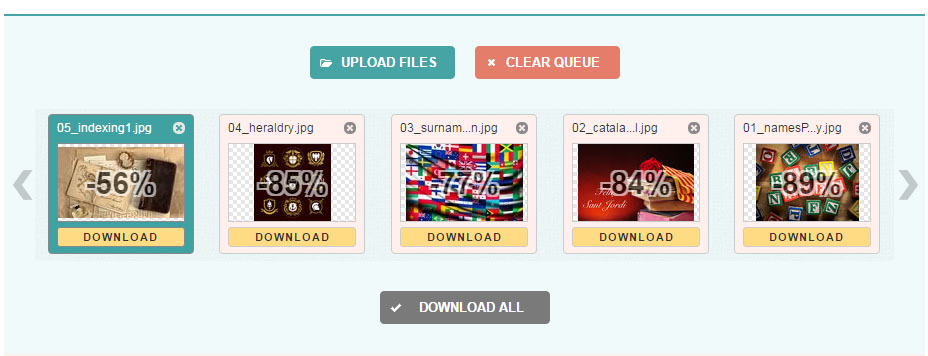
\includegraphics[width=\linewidth]{10/06_optimizilla}
        \centering
        \caption{Exemple d'optimització d'imatges mitjançant Optimizilla.}\label{img:optimizilla}
    \end{figure}
